%\begin{table*}
%\begin{center}
%\caption{\small{Monotonous stress intensity changes in U-SI and SI intervals compared with adjacent intervals.}}
%%\resizebox{\textwidth}{15mm}{
%\small{
%\begin{tabular}{l cccccc cccccc} \\\hline\hline
%\multirow{2}{1cm}{}
%&\multicolumn{2}{c}{School life}
%&\multicolumn{2}{c}{Romantic}
%&\multicolumn{2}{c}{Peer relationship}
%&\multicolumn{2}{c}{Self-cognition}
%&\multicolumn{2}{c}{Family life}
%&\multicolumn{2}{c}{All types}\\
%&U-SI	    &	SI	        &U-SI	    &SI	        &U-SI	   &SI	
%&U-SI	    &	SI	        &	U-SI	&SI	        &U-SI	   &SI\\  \hline
%\# Interval         &   365	        &	514	        &	536	        &	587	        &128	    &	391	        &	564	           &	609	            &	321	        &	481	        &	1,914	    &2,582	 \\
%Front $\rightarrow$ I &	0.7260 	&	0.7879 	&	0.6903 	&	0.7751 	&	0.7422 	&	0.8159 	&	0.7004 	&	0.7767 	&	0.6791 &	0.7796 	&	0.7017 	&   0.7851\\
%I $\rightarrow$ rear  &	0.7589 	&	0.7840 	&	0.7463 	&	0.7905 	&	0.7813 	&	0.8261 	&	0.7500 	&	0.7915 	&	0.7414 	&	0.7942 	&	0.7513 	&   0.7955\\ \hline \hline
%\end{tabular}}%}}
%\label{tab:fontrear}
%\end{center}
%\end{table*}
%
%\section{Results}
%In this section,
%%1.identify uplifts
%we first identify uplift events and corresponding restoring performance from microblogs,
%%2.identify restoring
%%3.identify scheduled restoring
%and compare the results with scheduled positive events collected from the school's official web site.

%4.predict
%Further, we integrate the impact of uplift events into traditional stress prediction in time line,
%and verify whether the restoring patterns of each type of uplift events could help improve the prediction performance,
%thus to show the effectiveness of our method for quantifying the impact of uplift events,
%as well as the easing function of uplift events during the process of dealing with stress.

%\subsection{Experimental setup}
%\subsubsection{Data set}
%We take the same data set in previous case study (section \ref{sec:obs}]),
%which contains 29,232 microblogs of 124 students from Taicang High School of Jiangsu Province from Tencent Microblog platform\footnote{http://t.qq.com/},
%posted from 2012/1/1 to 2015/2/1.
%To protect the privacy, all usernames are anonymized in the experiment.
%We collected the school's weekly plans published on its official web site.
%Among the 273 school scheduled events filtered out,
%122 events are study-related stressor events, and 75 are uplift events.
%Based on the scheduled time of stressor and uplift events,
%we identified 518 scheduled academic related stressful intervals (SI)
%and 259 academic stressful intervals impacted by four typical scheduled uplift events (U-SI) (in Table \ref{tab:schedule})
%from the students' microblogs.
%Further experiments are conducted on the two sets to verify the impact of uplift events from multi perspectives.

%\subsubsection{Baseline methods}
%To show the effectiveness,
%We adopt the commonly used Pearson correlation algorithms to compare with the two sample statistical method in this study.
%As a widely adopted measure of the linear correlation between two variables,
%the Pearson correlation method computes a value in the range ($-1,1$),
%where 1 denotes total positive linear correlation,
%0 denotes no linear correlation,
%and $-1$ is total negative linear correlation.
%The Pearson correlation between two variables \emph{X} and \emph{Y} is presented as:
%\begin{equation}
%\rho_{X,Y} = \frac{E[(X-\mu_X)(Y-\mu_Y)]}{\sigma_X\sigma_Y}
%\end{equation}
%where $\mu_X$ and $\mu_Y$ is the mean value of $X$ and $Y$, respectively;
%$E(.)$ is the expectation function;
%and $E[(X-\mu_X)(Y-\mu_Y)]$ is the covariance of the two variances $X$ and $Y$.

%In our two sample statistical procedure,
%to calculate the distance between two $n$ dimension points $X$ and $Y$,
%we adopt the $L_2$ measures,
%denoted as $L_2 = \sqrt{\sum_{i\in[1,n]}(X_i-Y_i)^2}$ (the Euclidean metric).

%\subsubsection{Metrics}
%To check the performance of uplift event extraction and the validation of our assumption,
%we first compare the experimental results with the school's scheduled positive events.

%Further, to measure the effectiveness of our method for quantifying the restoring impact of uplift events,
%we integrate the impact of uplift events into traditional stress series prediction problem,
%and verify whether the restoring pattern of uplift events could help improve the prediction performance.
%Here we choose the SVARIMA (Seasonal Autoregressive Integrated Moving Average) algorithm \cite{Shumway2006Time},
%which is proved to be suitable for teens' linear stress prediction problem \cite{Li2015Predicting},
%due to the seasonality and non-stationarity of teens' stress series.
%The basic stress prediction is conducted using SVARIMA approach,
%in the set of stressful intervals impacted by uplift events (U-SI).
%Since stressor events cause the fluctuation of stress series from normal states,
%%and the simple series prediction method is difficult to handle such exception.
%to eliminate the interference,
%we simply consider the prediction problem in those stressful intervals rather than randomly picked out stress series.
%Further, the impact of uplift events are utilized as adjust values to modify the stress prediction result.

%Four metrics are adopted to measure the stress forecasting problem,
%where \emph{MSE}, \emph{RMSE} and \emph{MAD} measure absolute errors and \emph{MAPE} measures relative errors.
%For all real stress value $\overline{s_i}$ and predicted stress value $s_i$ in predicting sequence $<s_1,\cdots,s_n>$,
%$MSE = \frac{1}{n}\sum_{i\in[1,n]}(s_i-\overline{s_i})^2$,
%$RMSE = \frac{1}{n}\sqrt{\sum_{i\in[1,n]}(s_i-\overline{s_i})^2}$,
%$MAD = \frac{1}{n}\sum_{i\in[1,n]}|s_i-\overline{s_i}|$,
%and $MAPE = \frac{1}{n}\sum_{i\in[1,n]}{|s_i-\overline{s_i}|/s_i}$.

\subsection{Impact and monotonous stress trends of uplift events}
%Basically, we focused on four kinds of scheduled positive events:
%\emph{practical activity}, \emph{holiday}, \emph{new year party} and \emph{sports meeting}.
%For each of the four scheduled positive events,
%we quantify the restoring impact and temporal order
%based on corresponding SI and U-SI interval sets of the 124 students.
%Table \ref{tab:schedule} shows the experimental results,
%where 54.52\%, 78.39\%, 63.39\%, 58.74\% significant restoring impact are detected for the four specific scheduled positive events, respectively, with the total accuracy to 69.52\%.
%For comparison,
%our knn-based two sample method (denoted as \emph{KTS}) outperforms the baseline method
%with the best improvement in \emph{new year party} to 10.94\%,
%and total improvement to 6\%.
%The correlation of uplift events for \emph{linguistic expression},
%\emph{stress intensity} and \emph{post behaviors} towards five types of stressor events
%are shown in Figure \ref{fig:correlation},
%among which the uplift events conduct most intensive restoring impact in 'school life' and 'peer relationship' dimensions.

%\begin{table}
%\begin{center}
%\caption{Quantify the impact of scheduled uplift school events using KTS and baseline method.}
%%\resizebox{\textwidth}{15mm}{
%\begin{tabular}{l c c c c c} \\ \hline \hline
%&	\emph{Practical}	&	         	&	\emph{New year}	&	\emph{Sports}	&	\emph{}	\\
%&	\emph{activity}	&	\emph{Holiday}	&	\emph{party}	&	\emph{meeting}	&	\emph{All}	\\ \hline
%Size of U-SI	&	219 	&	339 	&	235 	&	226 	&	1,019 	\\
%Pearson         &54.52\%	&	78.39\%	&	63.39\%	&	58.74\%	&	69.52\% \\
%KTS$^1$             &55.65\%	&	70.97\%	&	56.45\%	&	54.84\%	&	65.32\% \\
%\hline \hline
%\end{tabular}
%\begin{tablenotes}
%\footnotesize
%\item[1] $^1$KTS denotes the knn-based two sample method adopted in this research.
%\end{tablenotes}
%%}
%\label{tab:schedule}
%\end{center}
%\end{table}


%\begin{figure}
%\centering
%\caption{Correlation towards each types of stressor events}
%\includegraphics[width=\linewidth]{figs/correlation2.eps}%figs/correlation.eps
%\label{fig:correlation}
%\end{figure}
%
%\begin{table*}
%\caption{Compare the stress forecast performance under three restoring patterns of uplift events.}
%\begin{minipage}{\linewidth}
%\centering
%\resizebox{\textwidth}{15mm}{
%\begin{tabular}{l cccc cccc cccc cccc} \\\hline\hline%\toprule
%\multirow{2}{1cm}{}&\multicolumn{4}{c}{None}
%    &\multicolumn{4}{c }{Uplift (L)}
%    &\multicolumn{4}{c }{Uplift (S)}
%    &\multicolumn{4}{c}{Uplift (P)}\\
%    &\scriptsize{MSE} &\scriptsize{RMSE} &\scriptsize{MAPE} &\scriptsize{MAD}
%    &\scriptsize{MSE} &\scriptsize{RMSE} &\scriptsize{MAPE} &\scriptsize{MAD}
%    &\scriptsize{MSE} &\scriptsize{RMSE} &\scriptsize{MAPE} &\scriptsize{MAD}
%    &\scriptsize{MSE} &\scriptsize{RMSE} &\scriptsize{MAPE} &\scriptsize{MAD} \\\midrule					
%School life
%&   0.0856 	&	0.2926 	&	0.4852 	&	0.1146	&	0.0259 	&	0.1609 	&	0.2991 	&	0.0923 	
%&	0.0297 	&	0.1723 	&	0.3135 	&	0.0899 	&	0.0223 	&	0.1493 	&	0.3438 	&	0.0931 	\\
%Romantic
%&   0.0703 	&	0.2651 	&	0.3555 	&	0.1083 	&	0.0291 	&	0.1706 	&	0.2832 	&	0.0919 	
%&	0.0379 	&	0.1947 	&	0.2941 	&	0.1026 	&	0.0332 	&	0.0835 	&	0.2746 	&	0.1240 	\\
%Peer relationship
%&   0.2800 	&	0.5292 	&	0.3256 	&	0.1697 	&	0.3140 	&	0.5604 	&	0.3626 	&	0.1202 	
%&	0.2972 	&	0.5452 	&	0.3060 	&	0.1298 	&	0.2557 	&	0.1472 	&	0.3481 	&	0.1458 	\\
%Self-cognition
%&   0.0445 	&	0.2110 	&	0.3066 	&	0.1895 	&	0.0345 	&	0.1857 	&	0.2721 	&	0.1653 	
%&	0.0366 	&	0.1913 	&	0.2557 	&	0.0754 	&	0.0245 	&	0.0862 	&	0.2863 	&	0.1447 	\\
%Family life
%&   0.1602 	&	0.4002 	&	0.3291 	&	0.1587 	&	0.0889 	&	0.2982 	&	0.2891 	&	0.0944 	
%&	0.0378 	&	0.1944 	&	0.2952 	&	0.0842 	&	0.1827 	&	0.0979 	&	0.3148 	&	0.1131 	\\
%All	
%&   0.1281 	&	0.3579 	&	0.3604 	&	0.1482	&	0.0985 	&	0.3138 	&	0.3012 	&	0.1128 	
%&	0.0878 	&	0.2964 	&	0.2929 	&	0.0964 	&	0.1037 	&	0.1128 	&	0.3135 	&	0.1241 	\\ \hline\hline
%\end{tabular}}
%\end{minipage}\\
%\begin{minipage}{\linewidth}
%\centering
%\resizebox{\textwidth}{15mm}{
%\begin{tabular}{l cccc cccc cccc cccc} \\\hline\hline%\toprule
%\multirow{2}{1cm}{}&\multicolumn{4}{c}{Uplift (L\&S)}
%    &\multicolumn{4}{c }{Uplift (L\&P)}
%    &\multicolumn{4}{c }{Uplift (S\&P)}
%    &\multicolumn{4}{c}{Uplift (L\&S\&P)}\\
%    &\scriptsize{MSE} &\scriptsize{RMSE} &\scriptsize{MAPE} &\scriptsize{MAD}
%    &\scriptsize{MSE} &\scriptsize{RMSE} &\scriptsize{MAPE} &\scriptsize{MAD}
%    &\scriptsize{MSE} &\scriptsize{RMSE} &\scriptsize{MAPE} &\scriptsize{MAD}
%    &\scriptsize{MSE} &\scriptsize{RMSE} &\scriptsize{MAPE} &\scriptsize{MAD} \\\midrule					
%School life
%&	0.0283 	&	0.1682 	&	0.2934 	&	0.0824 	&	0.0261 	&	0.1616 	&	0.2770 	&	0.0768 	
%&	0.0342 	&	0.1849 	&	0.2629 	&	0.0590 	&	0.0132 	&	0.1149 	&	0.2364 	&	0.0717 	\\
%Romantic
%&	0.0219 	&	0.1480 	&	0.2532 	&	0.0839 	&	0.0180 	&	0.1342 	&	0.2644 	&	0.0952 	
%&	0.0176 	&	0.1327 	&	0.2549 	&	0.0823 	&	0.0251 	&	0.1584 	&	0.2507 	&	0.0891 	\\
%Peer relationship
%&	0.2361 	&	0.4859 	&	0.3182 	&	0.1300 	&	0.2349 	&	0.4847 	&	0.3283 	&	0.1189 	
%&	0.2351 	&	0.4849 	&	0.3558 	&	0.1297 	&	0.2341 	&	0.4838 	&	0.3096 	&	0.1093 	\\
%Self-cognition
%&	0.0329 	&	0.1814 	&	0.2942 	&	0.0946 	&	0.0262 	&	0.1619 	&	0.2791 	&	0.0858 	
%&	0.0245 	&	0.1565 	&	0.2740 	&	0.0945 	&	0.0144 	&	0.1200 	&	0.2580 	&	0.0739 	\\
%Family life
%&	0.1489 	&	0.3859 	&	0.2750 	&	0.1244 	&	0.0395 	&	0.1987 	&	0.2853 	&	0.0939 	
%&	0.0484 	&	0.2200 	&	0.2946 	&	0.0992 	&	0.0378 	&	0.1944 	&	0.2645 	&	0.0848 	\\
%All
%&	0.0936 	&	0.3060 	&	0.2868 	&	0.1031 	&	0.0689 	&	0.2626 	&	0.2868 	&	0.0941 	&	0.0720 	&	0.2683 	&	0.2884 	&	0.0929 	&	0.0649 	&	0.2548 	&	0.2638 	&	0.0858 	\\ \hline\hline
%\end{tabular}}
%\begin{tablenotes}
%        \footnotesize
%        \item[1] $^1$ Three restoring pattern measures: 'L' represents \emph{linguistic expression}, 'S' represents \emph{stress intensity}, and 'P' represents \emph{posting behavior}.
%      \end{tablenotes}
%\end{minipage}
%\label{tab:forecast}
%\end{table*}

%Further more,
%to verify the monotonous stress changes when an uplift event impacts a stressful interval,
%we collected 1,914 stressful intervals in U-SI,
%and 2,582 stressful intervals impacted by uplift events in SI.
%For each stressful interval in SI and U-SI,
%we quantify its stress intensity by comparing with the front and rear adjacent intervals, respectively.
%Here four situations are considered and compared according to the temporal order in Section \ref{sec:temporal},
%as shown in Table \ref{tab:fontrear},
%where the \emph{ratio of intervals} detected with monotonous increase from the \emph{front interval} to \emph{stressful interval} (denoted as \emph{front$ \rightarrow$ I}),
%and monotonous decrease from the \emph{stressful interval} to the \emph{rear interval} (denoted as \emph{I $\rightarrow$ rear}) are listed.
%Under the impact of uplift events,
%both the ratio of intensive stress increase in \emph{front$ \rightarrow$ I}
%and the ratio of intensive stress decrease in \emph{I $\rightarrow$ rear} are decreased,
%showing the effectiveness of the two sample method for quantifying the impact of uplift events,
%and the rationality of the assumption that uplift events could help ease stress of overwhelmed teens.

%\subsection{Integrate the impact of uplift events into stress forecasting}
%Next, we integrate the impact of uplift events into stress prediction.
%The experimental set contains 1,914 stressful intervals under the impact of uplift events (U-SI).
%The number of each type of uplift events and stressful intervals are lists in Table \ref{tab:fontrear}.
%As shown in Table \ref{tab:forecast},
%the original prediction result using only SVARIMA method
%achieves 0.1281 MSE, 0.3579 RMSE, 0.3604 MAPE and 0.1482 MAD ($L = 7$, $\alpha = 0.5$).
%Then we integrate the impact of each type of uplift events into stress prediction.
%Specifically, for uplifts with obvious restoring impact (under the L\&S\&P pattern),
%the average stress level during historical restoring intervals are integrated to modify the result,
%with adjusting the parameter $\alpha$ (details see \ref{sec:parameter}).
%After the modification,
%the prediction performance achieves 0.0649 MSE,	0.2548 RMSE, 0.2638 MAPE and 0.0858 MAD,
%reducing the prediction errors efficiently (with MSE, RMSE, MAPE and MAD reduced by 49.34\%, 28.81\%, 26.80\% and 42.11\%, respectively). %!!!!important result...

%Further,
%we present the prediction result under the impact of uplift events under different lengths of prediction windows,
%ranging from 1 to 10 days, as shown in \ref{fig:length}.
%With the window length increasing,
%the prediction error shows decreasing trend in all metrics.
%The reason is that longer prediction window takes more previous predicted results,
%and the error accumulates with more predicted values taken into the next step prediction.
%Among the five dimensions of events,
%the prediction for school life stress achieves the best performance.
%On one side,
%more uplift events and stressors about school life events are detected from teens microblogs,
%providing sufficient data in prediction.
%On the other side,
%stress coming from school life is the most common stress in the student group,
%with relative stable periodicity and high frequency.

%done
%\begin{figure}
%\centering
%\caption{Stress forecast performance under the L\&S\&P pattern of uplift events.}
%\includegraphics[width=\linewidth]{figs/threshNew.eps}
%\label{fig:thresh}
%\end{figure}

%\begin{figure*}
%\centering
%\caption{Teens' stress forecast performance under different lengths of predicting windows.}
%\includegraphics[width=\linewidth]{figs/predictWindow2.eps}
%\label{fig:length}
%\end{figure*}

%\subsection{Contribution of each restoring measure}
%We conduct experiments with different restoring patterns included respectively to show
%its contribution to the impact of uplift events during prediction.
%Four groups of situations are considered here, as shown in Table \ref{tab:forecast},
%considering
%1) all the stress intensity, linguistic expression and post behavior measures (the L\&S\&P pattern),
%2) any two of the three measures included (the L$|$S, L\&P, and S\&P patterns),
%3) only one of the three measures included (the L, S, or P patterns),
%and 4) none measure included.
%We integrate the impact of uplift events under the four situations into stress prediction
%using the parameter $\alpha$,
%as overlapping $\alpha \times S_{historical}$,
%where $S_{historical}$ is the average stress level in historical restoring intervals.
%The detailed adjust process of $\alpha$  is presenting in section \ref{sec:parameter}.
%Here we present the prediction result when $\alpha = 0.5$ in each dimension of stress respectively.
%Results show that the correlation in the L\&S\&P pattern outperforms other patterns
%(0.0649 MSE, 0.2548 RMSE, 0.2638 MAPE and 0.0858 MAD),
%showing the effectiveness of considering all the three correlations.

%\subsection{Parameter settings}
%\label{sec:parameter}
%The parameter $\alpha$ is adjusted when integrate the impact of uplift events into stress prediction.
%For each of the four groups of restoring patterns,
%we adjust $\alpha$ in the effect of $\alpha \times L$.
%We calculate the corresponding prediction result for each teen respectively,
%and show the result of the whole testing group using the averaging performance.
%Figure \ref{fig:thresh} shows the changing trend under the L\&S\&P pattern.
%The prediction error decreases first and then increases,
%and the best performance is achieved when $\alpha$ is nearby 0.52,
%with 0.0649 MSE, 0.2548 RMSE, 0.2638 MAPE and 0.0858 MAD as the average performance of the whole experimental data set.
%Multiple methods for integrating the impact of uplift event into stress prediction could be adopted.
%In this paper we adopt the simple one to verify the effectiveness of our model in quantifying the impact of uplift events,
%and the setting of parameter $\alpha$ could be changed due to different individuals and data sets.
